\documentclass[12pt]{beamer}
\usetheme{CambridgeUS}
\usepackage[utf8]{inputenc}
\usepackage[spanish]{babel}
\usepackage{amsmath}
\usepackage{multirow, array}
\usepackage{amsfonts}
\usepackage{amssymb}
\usepackage{graphicx}
\usepackage{ragged2e}
\setbeamertemplate{navigation symbols}{} 
\author[Kevin García - Alejandro Vargas]{Kevin García 1533173 \newline Alejandro Vargas 1525953}
\title[Diseños con medidas repetidas]{Diseño de experimentos con medidas repetidas}

%\setbeamercovered{transparent} 
%\setbeamertemplate{navigation symbols}{} 
%\logo{} 
%\institute{} 
%\date{} 
%\subject{} 
\begin{document}
\justifying
\begin{frame}[plain]
\maketitle
\end{frame}


\begin{frame}
\frametitle{Introducción}
En esta presentación veremos el concepto y aplicación de los diseños de medidas repetidas, pasando por las ventajas y desventajas que este presenta y por los nuevos conceptos que surgen en este tipo de diseño, como los efectos de orden (efecto de período y efecto residual) y el supuesto de esfericidad, además se mostrarán los distintos tipos de diseño de medidas repetidas que podríamos tener (simple, factorial y mixto) y se realizará un ejemplo para ilustrar su aplicación. 
\end{frame}

\begin{frame}
\frametitle{Diseño de medidas repetidas}
Cuando administramos los tratamientos objeto de investigación a los mismos sujetos y, en
consecuencia, estos reciben más de un tratamiento experimental, disponiendo al menos de una
observación por tratamiento y sujeto, decimos que estamos en presencia de un diseño intra-sujetos
o de medidas repetidas. Es decir, todos los sujetos de la muestra reciben todos los tratamientos.
De este modo, se trabaja con un solo grupo y cada individuo genera más de un dato. Estos diseños
constituyen una alternativa válida y en muchos casos más adecuada que los diseños entre-sujetos
o entre grupos.
\end{frame}

\begin{frame}
\frametitle{Diseño de medidas repetidas}
Estos diseños se pueden aplicar en diferentes tipos de situaciones, como:
\begin{itemize}
\justifying
\item Evaluación longitudinal del cambio a lo largo del tiempo.
\item Evaluación de la actuación de los sujetos bajo diferentes condiciones de tratamiento en
estudios transversales.
\end{itemize}
~\\Algunas de las ventajas del diseño de medidas repetidas son
\begin{itemize}
\justifying
\item Reducción radical del error experimental. Esto es así porque la variabilidad debida a las
diferencias individuales se elimina del término de error. De este modo, el diseño de medidas
repetidas constituye una estructura más potente para detectar el efecto del tratamiento que los
DCA (diseños completamente aleatorizados).
\end{itemize}
\end{frame}


\begin{frame}
\frametitle{Diseño de medidas repetidas}
\begin{itemize}
\justifying
\item Menor costo en número de sujetos, la reducción del número de sujetos es una ventaja
importante bajo múltiples punto de vista, incluidos el ahorro de tiempo y costos. Teniendo en
cuenta que el mismo grupo de sujetos recibe todos los tratamientos.
\item Incremento de la potencia del diseño. Es decir, dado que las diferencias entre los tratamientos
son valoradas dentro de cada sujeto y no entre los grupos, la variabilidad atribuida a las
diferencias individuales entre los sujetos, (efecto principal del factor sujetos), es eliminada del
término de error, aumentando con ello precisión y potencia de la prueba estadística y
acentuando así la validez de conclusión estadística \textbf{(Maxwell y Delaney, 1990; Vallejo, 1991)}.
\end{itemize}
\end{frame}

\begin{frame}
\frametitle{Diseño de medidas repetidas}
Algunas de las desventajas de este tipo de diseño son
\begin{itemize}
\justifying
\item El principal problema de los diseños de medidas repetidas son los efectos de orden que
derivan de la propia estructura del diseño. Estos efectos deben ser neutralizados para que no
confundan los efectos de los tratamientos. Pueden ser de dos tipos: efectos residuales y
efectos de período.
\item Los efectos de orden o la secuencia de administración de los tratamientos pueden sesgar los
resultados. Una de las posibles soluciones ante este problema puede ser contrabalanceo
equilibrando el orden de administración de los tratamientos mediante aleatorización de los
tratamientos.
\end{itemize}
\end{frame}

\begin{frame}
\frametitle{Diseño de medidas repetidas}
\begin{itemize}
\justifying
\item Otro inconveniente es la posible violación de algún supuesto de naturaleza estadística. Puesto que son los mismos sujetos los
que reciben cada una de las condiciones experimentales es normal que en estos diseños
aparezca un efecto sistemático en las respuestas, dando lugar a la aparición de correlación o
dependencia entre los errores, algo por lo demás muy habitual en estos diseños \textbf{(Winer, 1971)}.
La violación de este supuesto repercute gravemente en los resultados obtenidos, ya que la
prueba F no es robusta ante observaciones correlacionadas o dependientes.
\item Otra desventaja que tienen estos diseños es que en la presencia de datos missing en alguna
observación se deben tomar acciones: 1) Eliminar el sujeto del análisis: 2) Utilizar métodos de
imputación.
\end{itemize}
\end{frame}

\begin{frame}
\frametitle{Efectos de orden}
Como se mencionó anteriormente, existen dos tipos de efectos de orden.
\begin{itemize}
\justifying
\item Efecto de período: Los efectos de período ocurren cuando, independientemente del tratamiento aplicado, el sujeto responde al período o posición que, en la secuencia, ocupa el tratamiento (período de administración). Cabe, por lo tanto, la posibilidad de que el sujeto responda mejor al período que al tratamiento en sí mismo. Cuando esto ocurre, el efecto de período confunde la acción del tratamiento.

~\\\textbf{Solución:} Contrabalanceo o aleatorización de los tratamientos.
\end{itemize}
\end{frame}

\begin{frame}
\frametitle{Efectos de orden}
\begin{itemize}
\justifying
\item Efecto residual: El efecto residual, conocido por error progresivo, se caracteriza por la persistencia de la acción de un tratamiento más allá del período o tiempo de aplicación. Representa la progresiva acumulación tanto de los efectos facilitadores de la respuesta (efecto de la práctica, aprendizaje, etc.) como de los efectos obstaculizadores (como la fatiga mental, cansancio físico, etc.).
~\\Cuando, como es frecuente en esos casos, se produce una persistencia del efecto del tratamiento anterior sobre el tratamiento siguiente, se corre el riesgo de que los efectos queden contaminados.

~\\\textbf{Solución:} Aumentar el intervalo de tiempo entre un tratamiento y el siguiente.                                  
\end{itemize}
\end{frame}

\begin{frame}
\frametitle{Supuestos}
El adecuado análisis de los diseños de medidas repetidas requiere el cumplimiento de ciertos
supuestos que aseguren la validez del contraste de hipótesis mediante la prueba F. Se asume la
homogeneidad de las varianzas intra- tratamiento (esfericidad), y se asume que las observaciones
en los diferentes niveles del tratamiento siguen una distribución normal conjunta multivariada. La
violación de alguno de estos supuestos afectará al error de Tipo I y a la potencia de la prueba F; de
entre ellos es especialmente grave la existencia de correlación entre los errores \textbf{(Winer, 1971;
Kirk, 1982)}.
\end{frame}

\begin{frame}
\frametitle{Supuestos}
El principal supuesto es el de esfericidad, que consta de homogeneidad o igualdad de las
varianzas de las diferencias entre pares de puntuaciones. \textbf{(Huynt y Feldt 1970) y Rouanet y
Lépine (1970)} demostraron que la homogeneidad de las varianzas de las diferencias equivale a
asumir que la matriz de covarianza tiene determinada forma, denominada esfericidad o
circularidad.

~\\Existen procedimientos que permiten comprobar la hipótesis nula de
esfericidad (la igualdad u homogeneidad de las varianzas poblacionales de las puntuaciones de
diferencia). Una de ellas es la prueba W de Mauchly (1940) .
\end{frame}

\begin{frame}
\frametitle{Clasificación}
La clasificación del diseño de medidas repetidas en función de los grupos es:
\begin{itemize}
\item Diseño de medidas repetidas simple
\item Diseño de medidas repetidas factorial
\item Diseño de medidas repetidas factorial mixto
\end{itemize}
~\\En esta presentación se analizará el diseño de medidas repetidas simple, ya que es el más sencillo de entender y a partir del análisis de este se podrían obtener los demás.
\end{frame}

\begin{frame}
\frametitle{Diseño de medidas repetidas simple}
La estructura del diseño de medidas repetidas simple es similar a la estructura de un diseño
factorial de dos variables independientes. A diferencia del diseño factorial, la variable de sujetos no
es manipulada ya que se trata de un pseudo-factor. La variable de tratamientos está manipulada
por el experimentador y es considerada como un auténtico factor.
\end{frame}

\begin{frame}
\frametitle{Diseño de medidas repetidas simple}
Esta estructura está dada por:
$$y_{ij}=\mu+\tau_i+\alpha_j+\varepsilon_{ij} \;\;\;\; i=1,...,t \;\;\;  \wedge \;\;\; j=1,...,r$$
$y_{ij}:$ Valor de la variable de respuesta del sujeto j bajo el tratamiento i.

$\mu:$ Media general sin tener en cuenta el sujeto ni el tratamiento.

$\tau_i:$ Efecto del i-ésimo tratamiento en la variable de respuesta.

$\alpha_j:$ Efectos del j-ésimo sujeto en la variable de respuesta.

$\varepsilon_{ij}:$ Error aleatorio debido al i-ésimo tratamiento y al j-ésimo sujeto.

\textbf{Supuestos:} 
$$\alpha_j \simeq N(0,\sigma^2_\alpha)$$
$$\varepsilon_{ij} \simeq N(0,\sigma^2_\varepsilon)$$
$$\Sigma =\sigma^2 11' + \sigma^2_\varepsilon I$$
\end{frame}

\begin{frame}
\frametitle{Análisis de varianza}
En el análisis de varianza correspondiente para este tipo de diseño, se evalúan dos hipótesis esencialmente:
~\\La hipótesis principal es la de los tratamientos
\begin{center}
~\\$H_0:\tau_1=\tau_2=\cdots=\tau_t=\tau$
~\\$H_1:$Al menos una de estas igualdades no se cumple.
\end{center}
~\\También existe interés en determinar si existen diferencias entre los sujetos
\begin{center}
~\\$H_0:\alpha_1=\alpha_2=\cdots=\alpha_r=\alpha$ 
~\\$H_1:$Al menos una de estas igualdades no se cumple.
\end{center}
\end{frame}

\begin{frame}
\frametitle{Análisis de varianza}
~\\Las hipótesis anteriores se pueden probar realizando el análisis de varianza como sigue:

\begin{table}[htbp]
  \centering
\resizebox{12cm}{!} {
\begin{tabular}{|c|c|c|c|c|c|c|}
\hline 
\parbox{7em}{\centering Fuente\\ de Variación} & \parbox{7em}{\centering Grados de\\ Libertad} & Suma de Cuadrados & Cuadrados Medios & F & $Pr>F$ & ECM \\ 
\hline 
Tratamientos & $t-1$ & $\sum\limits_{i=1}^{t}\frac{y^2_{i.}}{r}-\frac{(y_{..})^2}{tr}$ & $CM_\tau=\frac{SC_\tau}{t-1}$ & $\frac{CM_{\tau}}{CM_{error}}$ &  & $r\sum\limits_{i=1}^{t}\frac{(\tau_i-\bar{\tau_{.}})^2}{t-1}+\sigma^2$\\ 
Sujetos & $r-1$ & $\sum\limits_{j=1}^{r}\frac{y^2_{.j}}{t}-\frac{(y_{..})^2}{tr}$ & $CM_\alpha=\frac{SC_\alpha}{r-1}$ & $\frac{CM_{\alpha}}{CM_{error}}$ & &$t\sum\limits_{j=1}^{r}\frac{(\alpha_{j}-\bar{\alpha_{.}})^2}{r-1}+\sigma^2$ \\
Error & $(t-1)(r-1)$ & $\vec{y'}\vec{y}-\sum\limits_{i=1}^{t}\frac{y^2_{i.}}{r}-\sum\limits_{j=1}^{r}\frac{y^2_{.j}}{t}+\frac{(y_{..})^2}{tr}$ & $CM_{error}=\frac{SC_{error}}{(t-1)(r-1)}$ &   & & $\sigma^2$\\ 
Total & $tr-1$ & $\vec{y'}\vec{y}-\frac{(y_{..})^2}{tr}$ &  &   & &\\ 
\hline 
\end{tabular} 
}
\caption{ANOVA}
\label{tab:addlabel}%
\end{table}%
\end{frame}

\begin{frame}
\frametitle{Ejemplo}
Un total de 5 ratas son pesadas cuatro veces con intervalos de 4 semanas (semana 8, 12, 16 y 20). El objetivo es determinar el efecto del tiempo sobre el peso en gramos de las ratas. Los datos se presentan a continuación:
\begin{table}[htbp]
  \centering
\resizebox{12cm}{!} {
\begin{tabular}{|c|c|c|c|c|}
\hline 
\textbf{Rata} & \textbf{Semana 8} & \textbf{Semana 12} & \textbf{Semana 16} & \textbf{Semana 20}\\ 
\hline 
1 & 164 &220& 261& 306\\
2 & 164 &230& 275& 326\\
3 &158 &226& 264& 320\\
4 &159 &227& 280& 330\\
5 &155 &222 &272& 312\\
\hline 
\end{tabular} 
}
\caption{Datos ejemplo}
\label{tab:addlabel}%
\end{table}%
\end{frame}

\begin{frame}
\frametitle{Ejemplo}
\begin{itemize}
\item Factor: Tiempo
\item Niveles: Semana 8, semana 12, semana 16 y semana 20
\item Factor sujeto: Rata
\item Variable de respuesta: Peso en gramos de las ratas
\end{itemize}
Modelo estadístico asociado:
\begin{center}
$y_{ij}=\mu+\tau_i+\alpha_j+\varepsilon_{ij} \;\;\;\; i=1,...,4 \;\;\;  \wedge \;\;\; j=1,...,5$
\end{center}
$y_{ij}:$ Peso en gramos de la rata j en la semana i.

$\mu:$ Peso promedio sin tener en cuenta las ratas ni las semanas.

$\tau_i:$ Efecto de la i-ésima semana en el peso de la rata.

$\alpha_j:$ Efecto de la j-ésima rata en el peso.

$\varepsilon_{ij}:$ Error aleatorio debido a la rata j-ésima en la semana i-ésima.

\end{frame}

\begin{frame}
\frametitle{Ejemplo}
\textbf{Supuestos:} 
$$\alpha_j \simeq N(0,\sigma^2_\alpha)$$
$$\varepsilon_{ij} \simeq N(0,\sigma^2_\varepsilon)$$
$$\Sigma =\sigma^2 11' + \sigma^2_\varepsilon I$$

\textbf{Descriptivas:}
\begin{table}[htbp]
  \centering
\resizebox{12cm}{!} {
\begin{tabular}{|c|c|c|c|c|c|}
\hline 
\textbf{Tiempo} & \textbf{$\bar{X}$} & \textbf{$S$} & \textbf{$CV(\%)$} & \textbf{$Min$} & \textbf{$Max$}\\ 
\hline 
Semana 8 & 160 &3.937004& 2.46& 155 & 164\\
Semana 12 & 225 &4& 1.77& 220 & 230\\
Semana 16 & 270.4 &7.829432& 2.89& 261 & 280\\
Semana 20 & 318.8 &9.859006& 3.09& 306 & 330 \\
\hline 
\end{tabular} 
}
\caption{Descriptivas por tratamientos}
\label{tab:addlabel}%
\end{table}%
\end{frame}

\begin{frame}
\frametitle{Ejemplo}
\begin{table}[htbp]
  \centering
\resizebox{12cm}{!} {
\begin{tabular}{|c|c|c|c|c|c|}
\hline 
\textbf{Tiempo} & \textbf{$\bar{X}$} & \textbf{$S$} & \textbf{$CV(\%)$} & \textbf{$Min$} & \textbf{$Max$}\\ 
\hline 
Rata 1 & 237.75 &60.42282 & 25.41& 164 & 306\\
Rata 2 & 248.75 &68.77681 & 27.65& 164 & 326\\
Rata 3 & 242    &68.01961 & 28.10& 158 & 320\\
Rata 4 & 249    &73.27119 & 29.42& 159 & 330 \\
Rata 5 & 240.25 &67.71694 & 28.18& 155 & 312 \\
\hline 
\end{tabular} 
}
\caption{Descriptivas por sujetos}
\label{tab:addlabel}%
\end{table}%
\end{frame}

\begin{frame}
\frametitle{Ejemplo}
\begin{figure}[h!]
\caption{Diagrama de cajas de los pesos(gramos) por semanas}
  \centering
  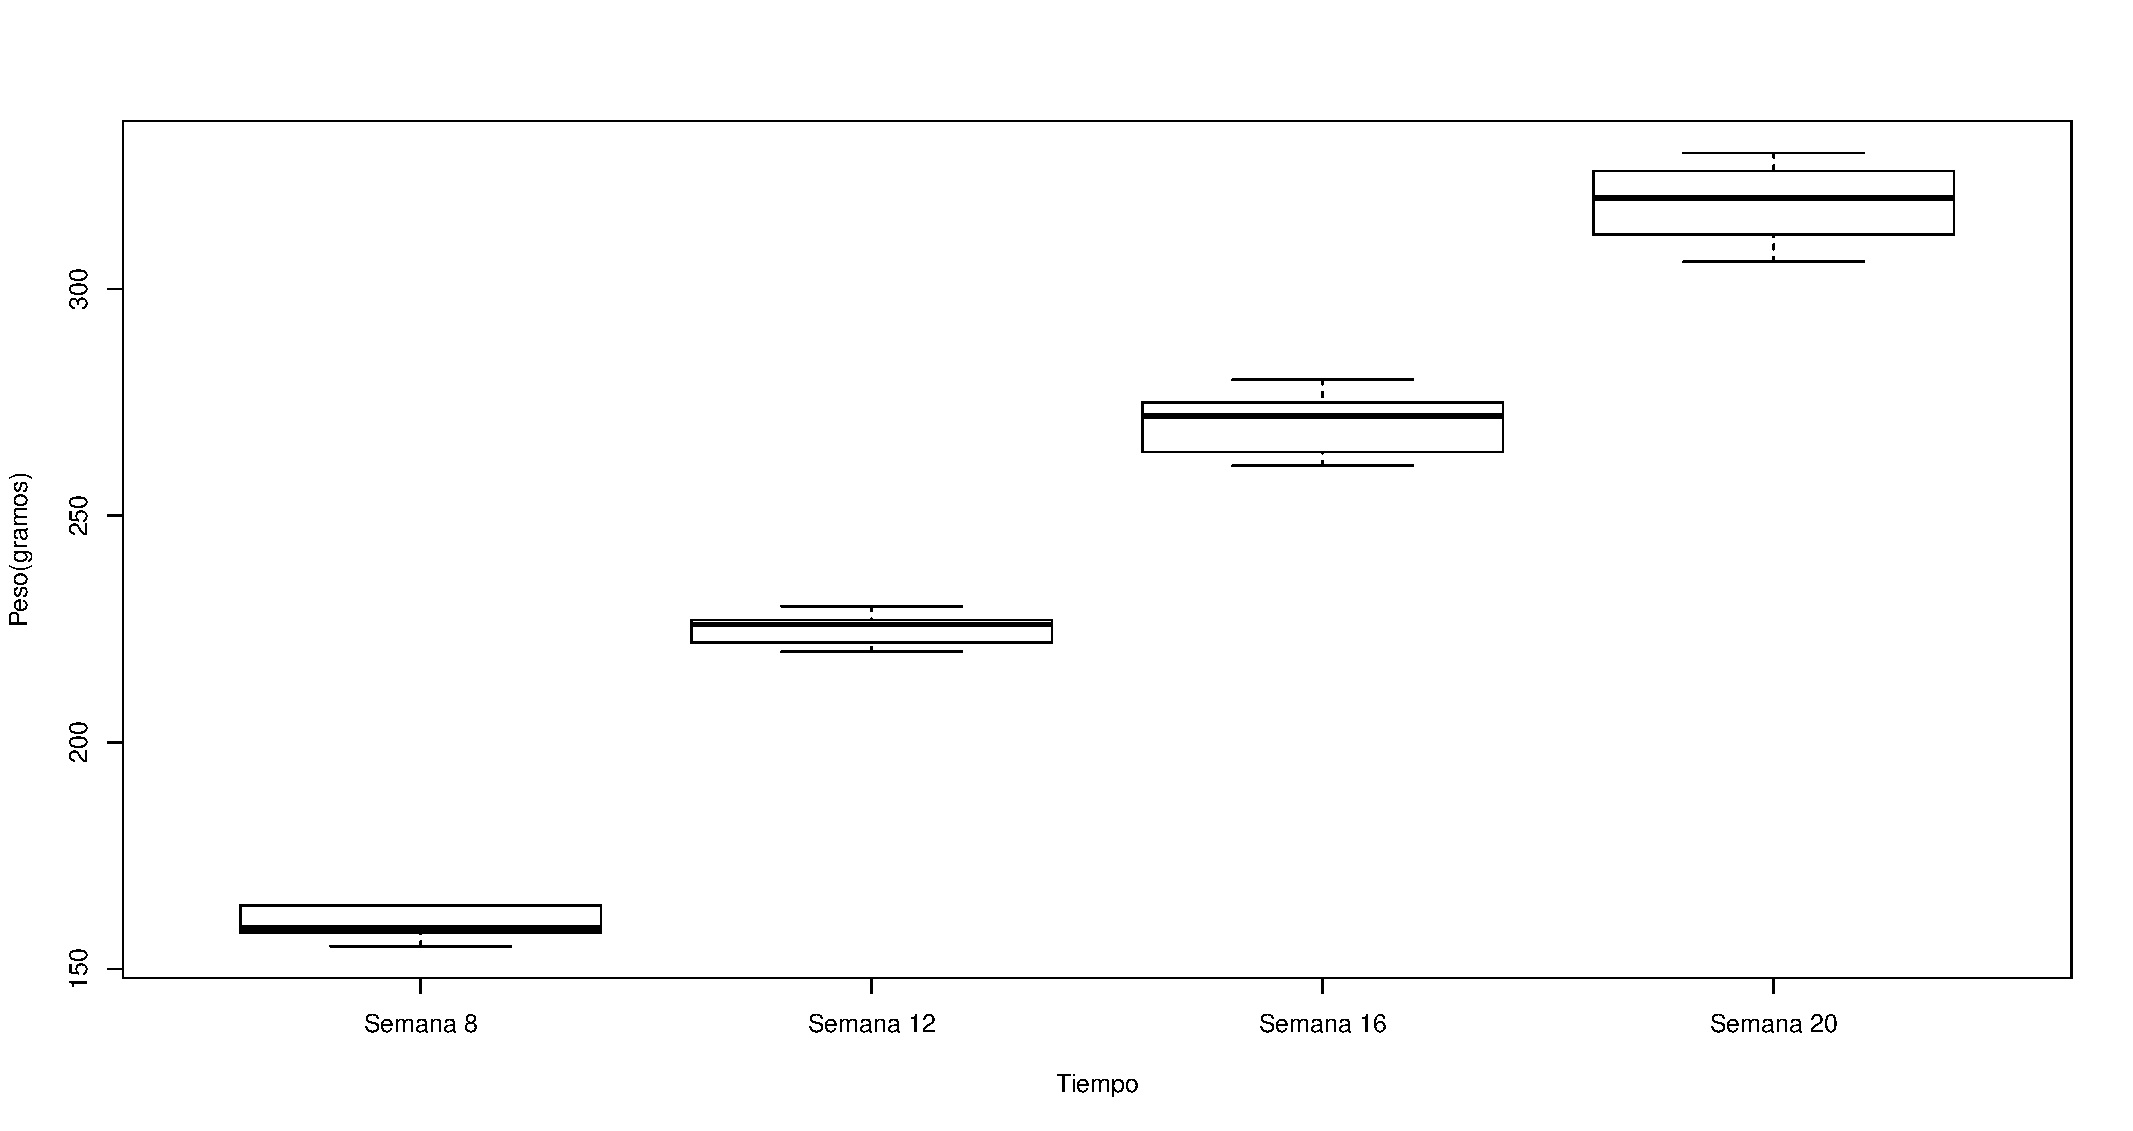
\includegraphics[scale=0.33]{imagenes/D.pdf}
\end{figure}
\end{frame}

\begin{frame}
\frametitle{Ejemplo}
\begin{figure}[h!]
\caption{Diagrama de cajas de los pesos(gramos) por rata}
  \centering
  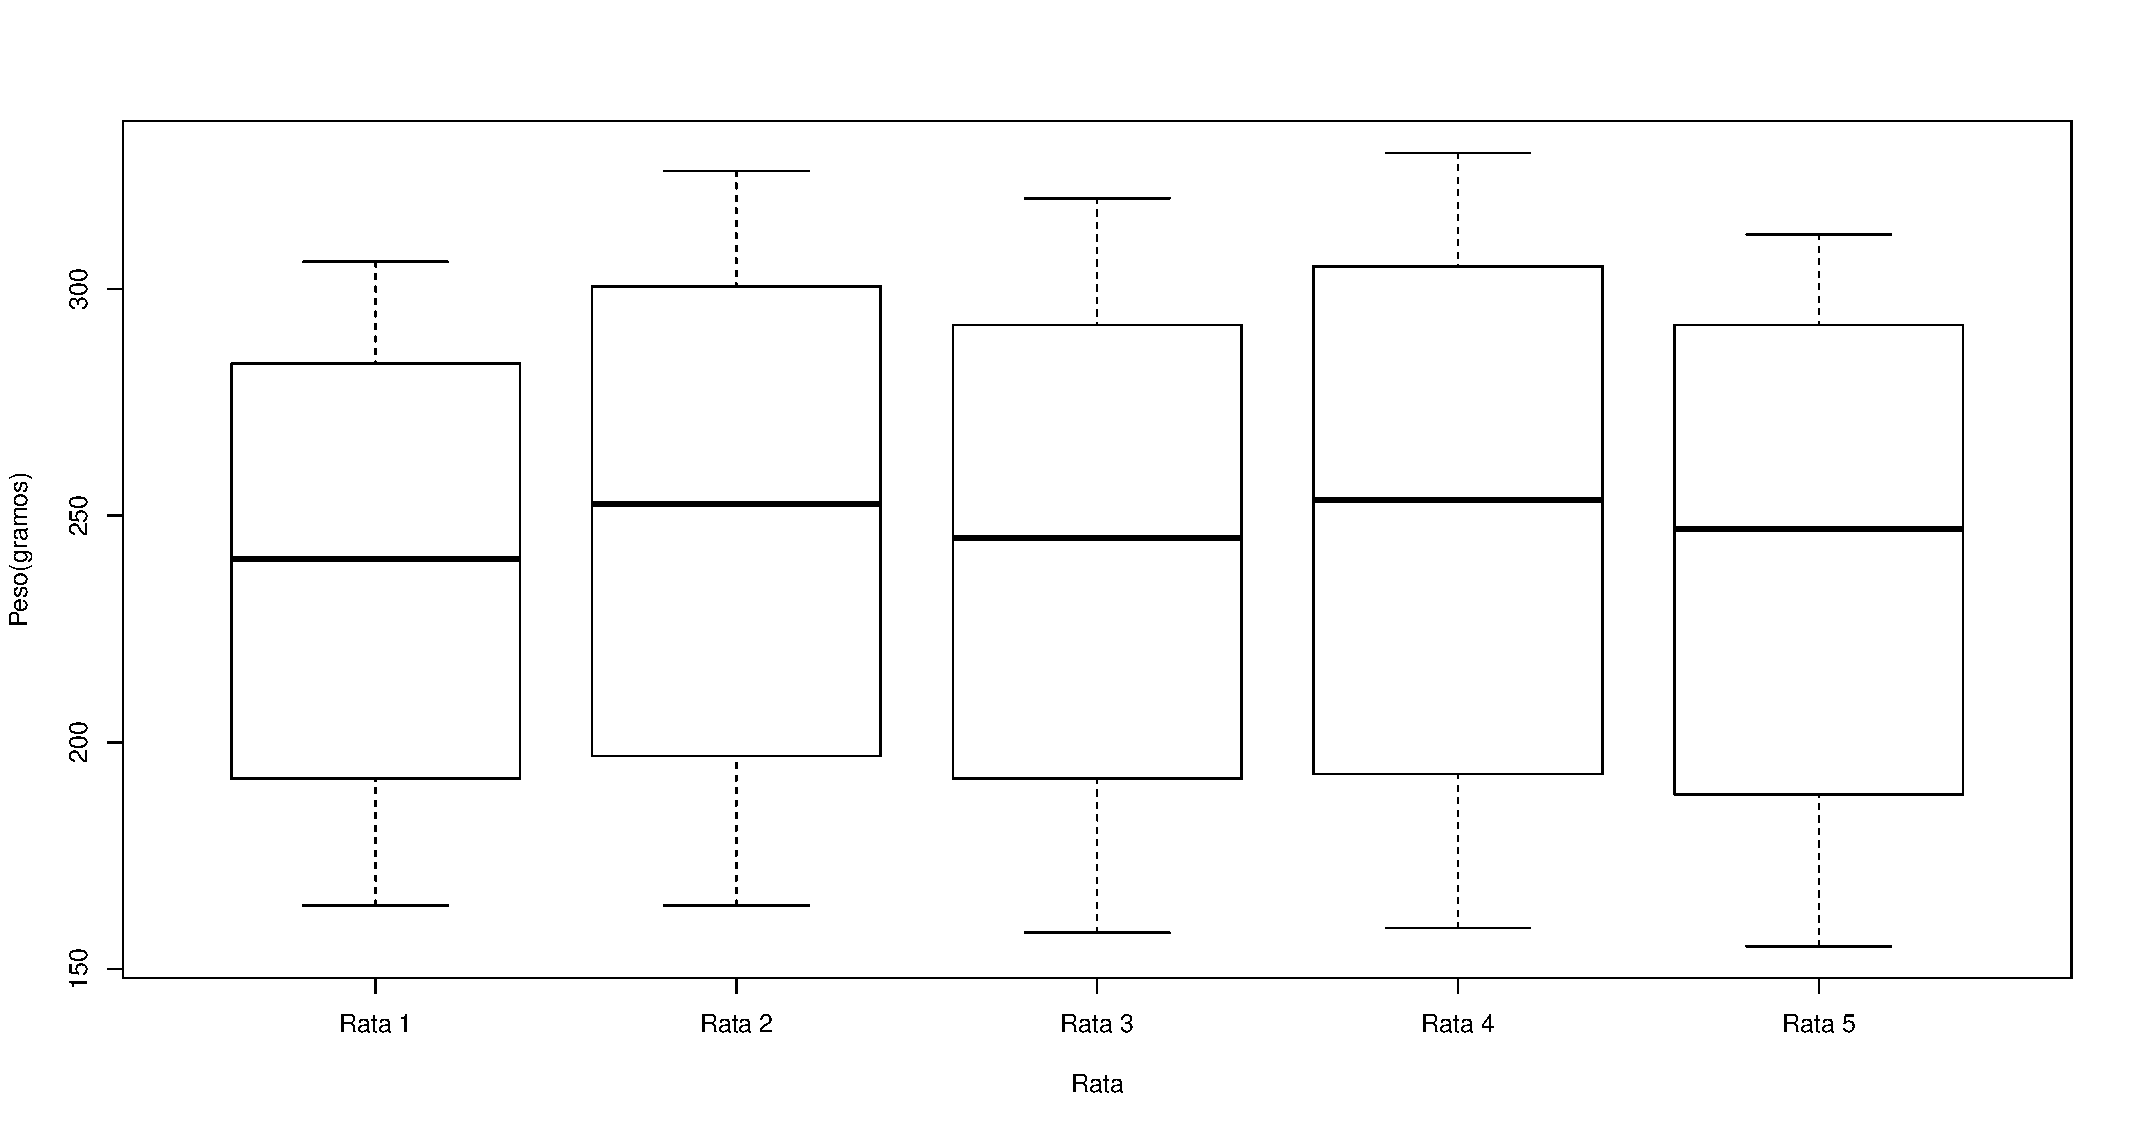
\includegraphics[scale=0.33]{imagenes/D1.pdf}
\end{figure}
\end{frame}

\begin{frame}
\frametitle{Ejemplo}
\begin{figure}[h!]
\caption{Tendencia del peso por rata}
  \centering
  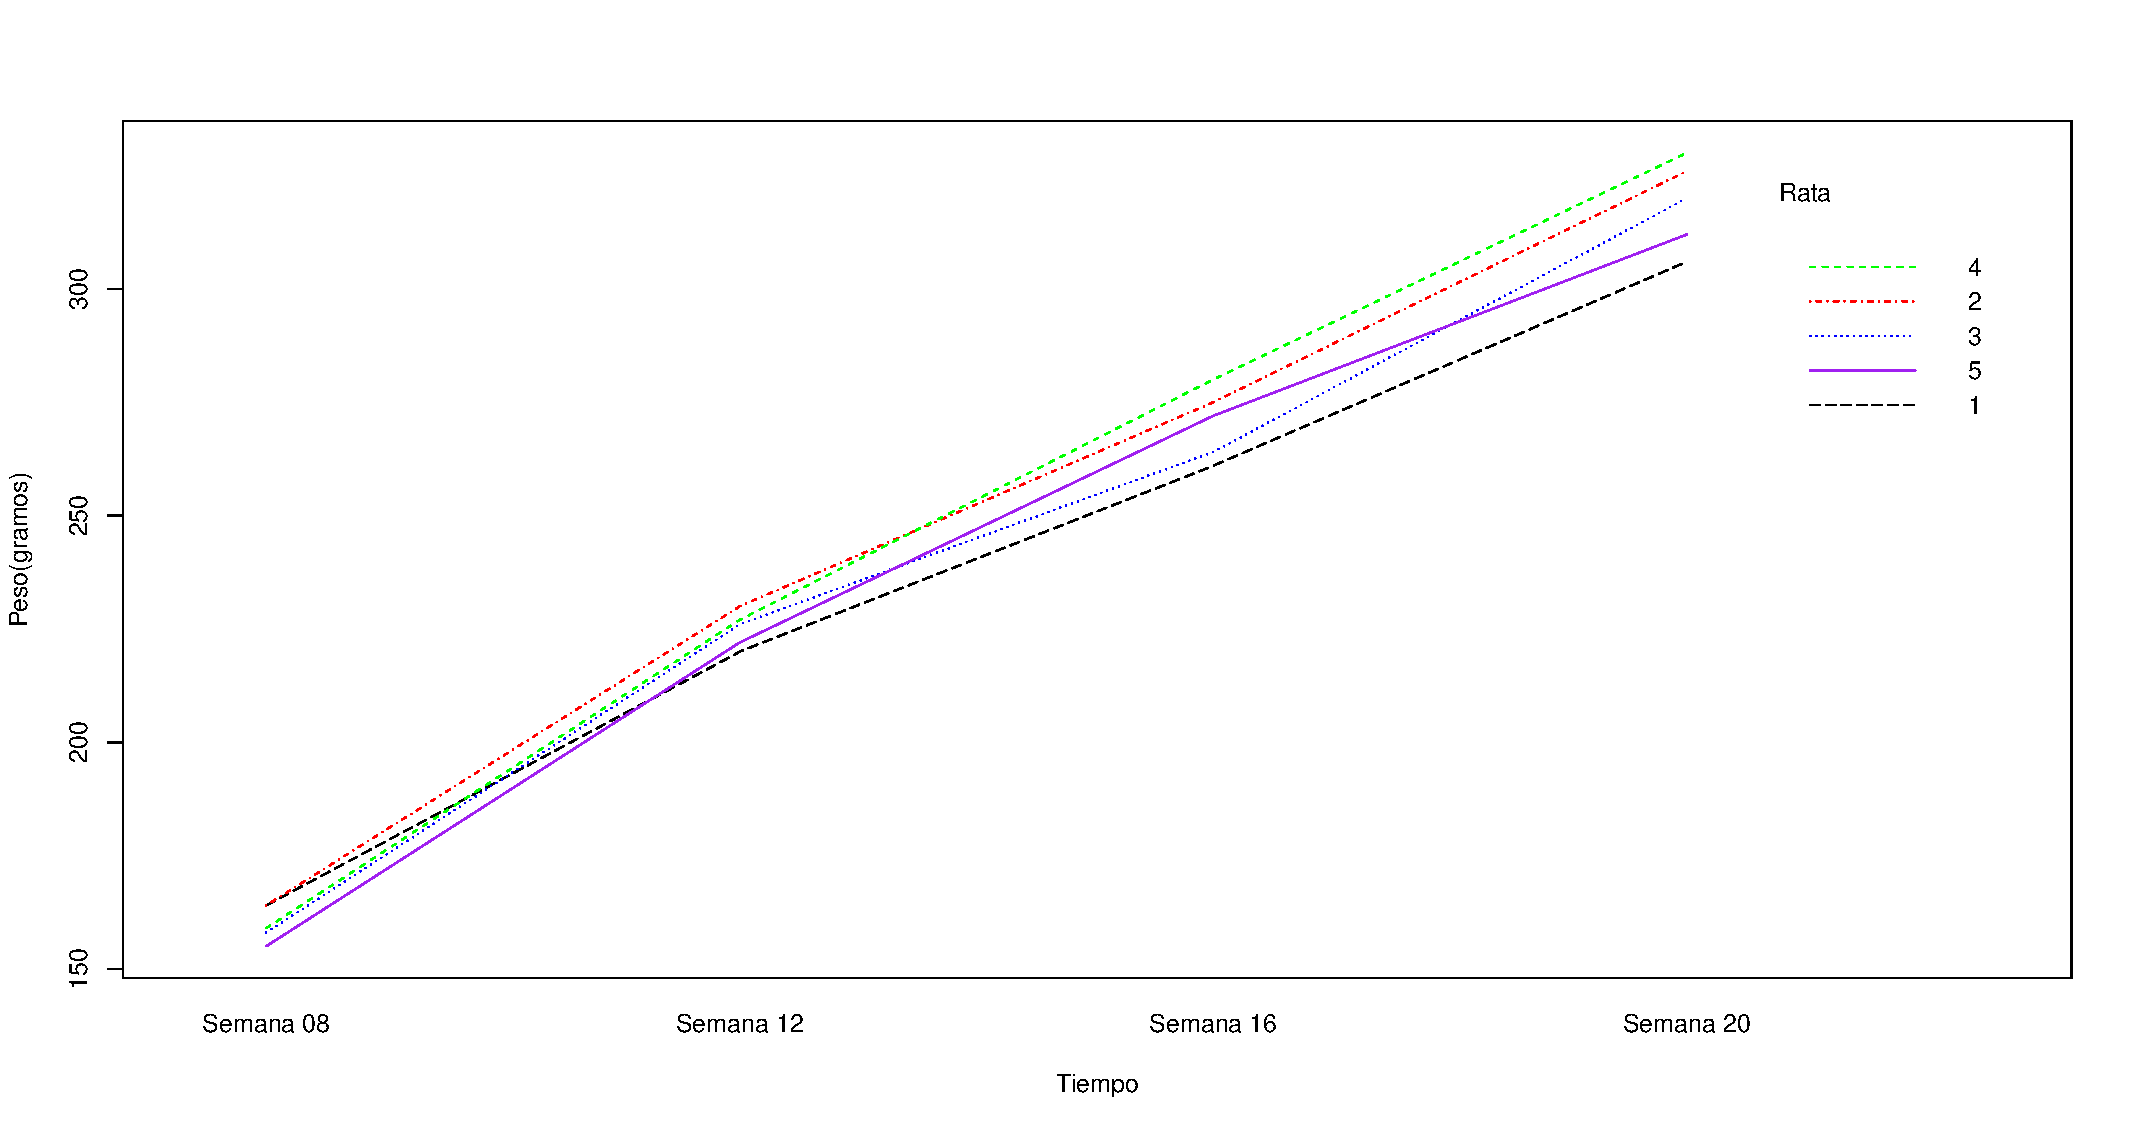
\includegraphics[scale=0.33]{imagenes/I.pdf}
\end{figure}
\end{frame}

\begin{frame}
\frametitle{Ejemplo}
Primero verificamos los supuestos para poder realizar adecuadamente el análisis de varianza. 
 $$\alpha_j \simeq N(0,\sigma^2_\alpha)$$

Para validar este supuesto se utilizó la prueba Shapiro Wilk ya que se tienen muestras pequeñas.
~\\\textbf{Resultados:}
\begin{itemize}
\item[]Semana 8 \textbf{valor-p =0.359}
\item[]Semana 12 \textbf{valor-p =0.833}
\item[]Semana 16 \textbf{valor-p =0.7556}
\item[]Semana 20 \textbf{valor-p =0.8154}
\end{itemize}
A un nivel de significancia del 5\% No rechazamos la hipótesis nula para ninguno de los casos, es
decir que hay evidencia muestral para pensar que se cumple la normalidad intra-sujetos.
\end{frame}

\begin{frame}
\frametitle{Ejemplo}
Ahora realizamos la prueba de esfericidad por medio del test de Mauchly para observar si hay o no
esfericidad en la matriz $\Sigma$ bajo las siguientes hipótesis.
\begin{center}
$H_0$: Hay esfericidad.

$H_1$: No hay esfericidad.
\end{center}
\textbf{Resultados:}
\begin{figure}[h!]
  \centering
  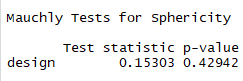
\includegraphics[scale=0.8]{imagenes/TM.png}
\end{figure}
A un nivel de significancia del 5\% no rechazamos Ho, por lo tanto podemos concluir que se cumple
el supuesto de esfericidad, es decir que no hay diferencias en las varianzas para todos los pares
de grupos.
\end{frame}

\begin{frame}
\frametitle{Ejemplo}
Finalmente, se probó el supuesto de normalidad en los errores:
\begin{figure}[h!]
  \centering
  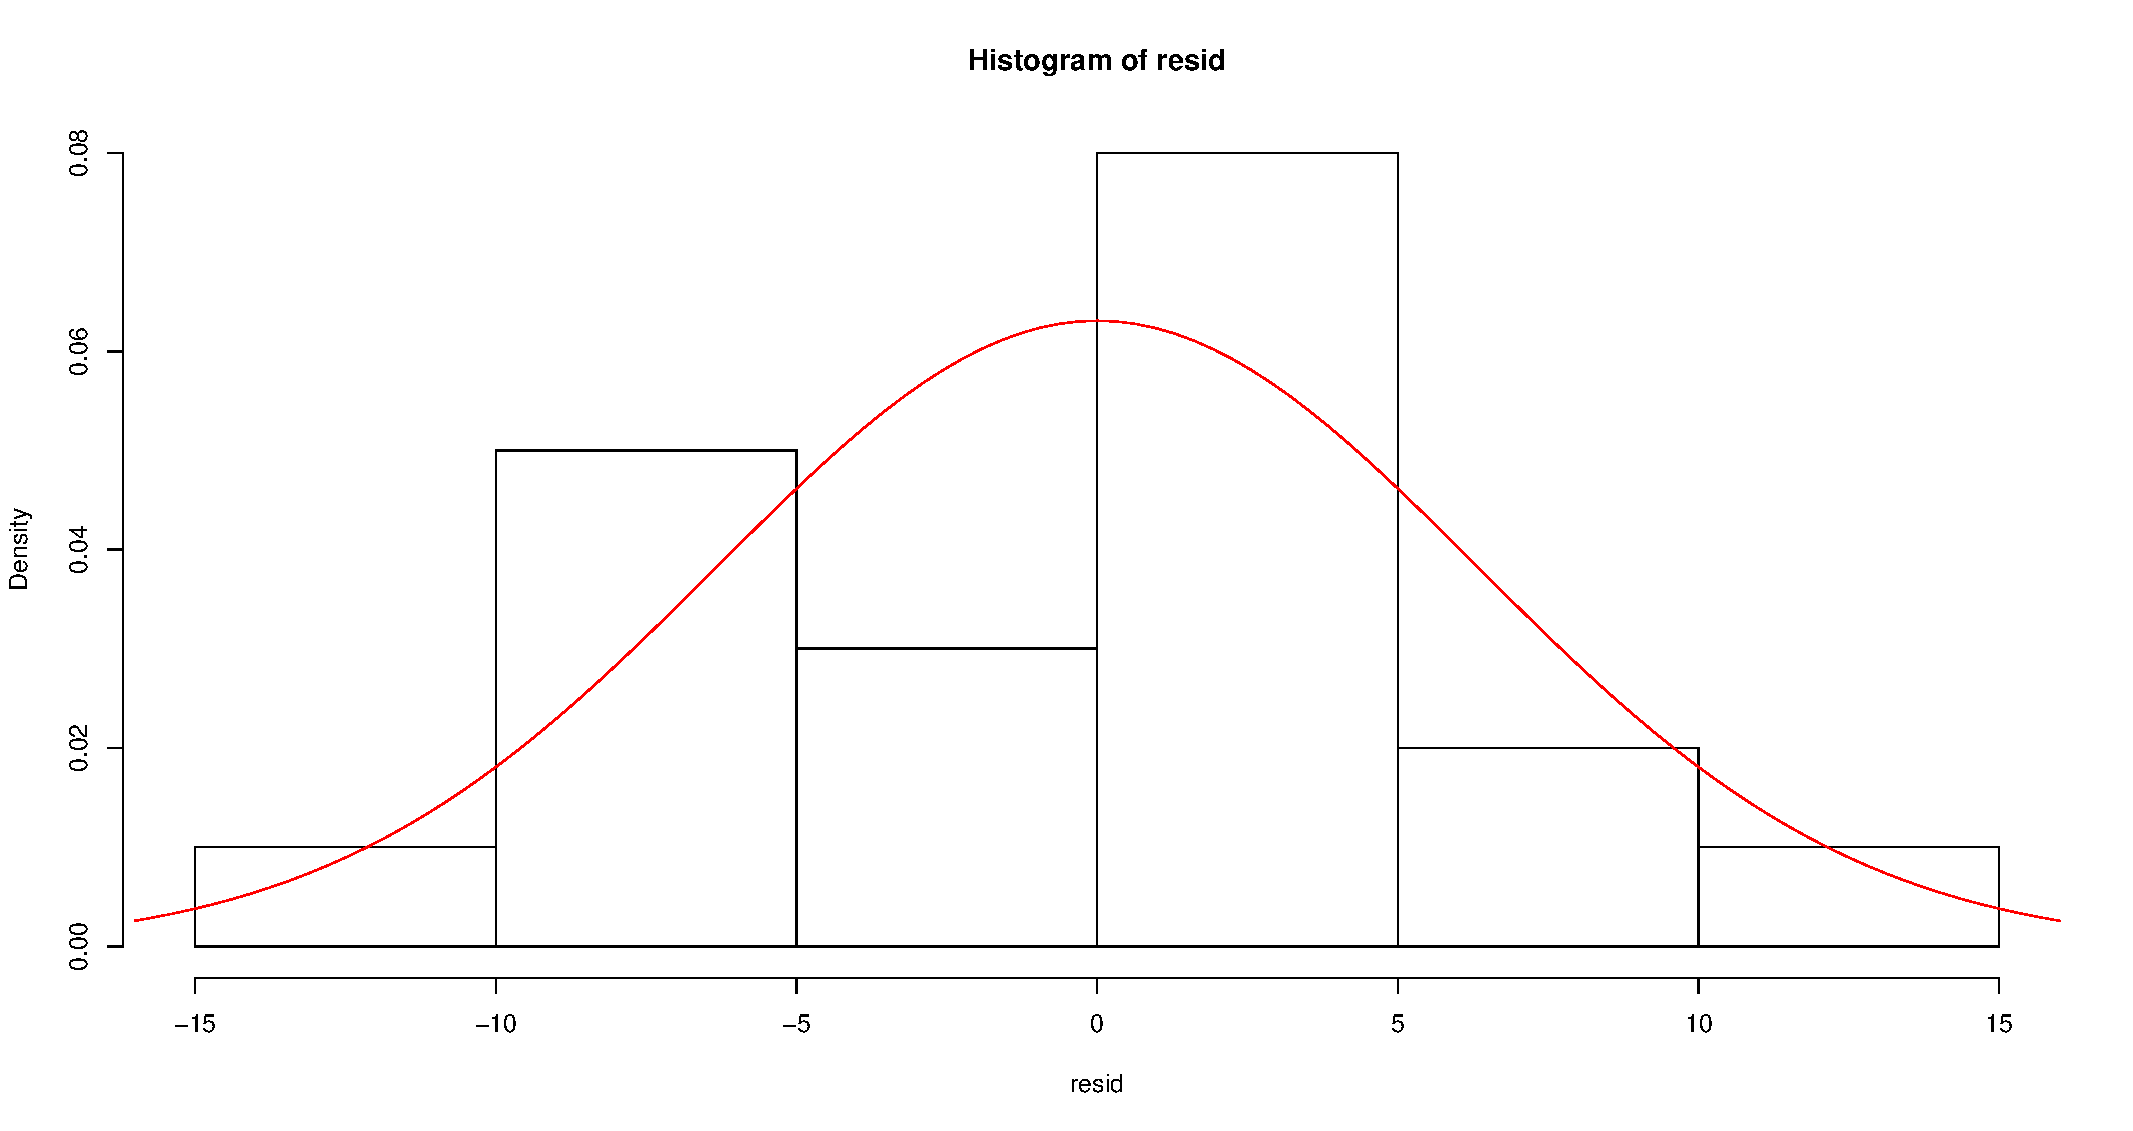
\includegraphics[scale=0.3]{imagenes/N.pdf}
\end{figure}
Y, la prueba Shapiro Wilk tuvo un p-valor =0.9801.
\end{frame}

\begin{frame}
\frametitle{Ejemplo}
Luego de probar todos los supuestos, podemos confiar en que el análisis de varianza obtenido es válido.

\textbf{Hipótesis}
\begin{center}
$H_0:\tau_1=\tau_2=\cdots=\tau_t=\tau \;\;\;\; \wedge \;\;\;\; H_0:\alpha_1=\alpha_2=\cdots=\alpha_r=\alpha $

$H_1:$Al menos una de estas igualdades no se cumple.
\end{center}
\begin{table}[htbp]
  \centering
\resizebox{10cm}{!} {
\begin{tabular}{|c|c|c|c|c|c|c|}
\hline 
\parbox{7em}{\centering Fuente\\ de Variación} & \parbox{7em}{\centering Grados de\\ Libertad} & Suma de Cuadrados & Cuadrados Medios & F & $Pr>F$ & ECM \\ 
\hline 
Tiempo & 3 & 68541 & 22847 & 794 & 4.64e-14  & $r\sum\limits_{i=1}^{t}\frac{(\tau_i-\bar{\tau_{.}})^2}{t-1}+\sigma^2$\\ 
Rata & 4 & 414.7 & 103.7 & 3.6 & 0.03759 &$t\sum\limits_{j=1}^{r}\frac{(\alpha_{j}-\bar{\alpha_{.}})^2}{r-1}+\sigma^2$ \\
Error & 12 & 345.3 & 28.775 &   & & $\sigma^2$\\ 
Total & 19 & 69300.95 &  &   & &\\ 
\hline 
\end{tabular} 
}
\caption{ANOVA Ejemplo}
\label{tab:addlabel}%
\end{table}%
Podemos concluir que existen diferencias entre los efectos del tiempo(semanas) sobre el peso de las ratas a un nivel de
significancia del 5\%.
\end{frame}


%-----------------------------------------------------------
\begin{frame}
\frametitle{Referencias}
\begin{itemize}
\item Kuehl, R. O. (2001), Diseño de experimentos

\item Montgomery, D. C. (2004), Diseño y análisis de experimentos.

\item Llobell, J. P., Navarro, M. D. F., \& Pérez, J. F. G. (1996). Manual de psicología experimental.

\item Arnau, J. (2007). Estudios longitudinales de medidas repetidas. Modelos de diseño y de análisis. 

\item Fox, J. \&  Weisberg, S. (2011). An {R} Companion to Applied Regression.
*http://socserv.socsci.mcmaster.ca/jfox/Books/Companion
\end{itemize}
\end{frame}

\end{document}